    Let $\DT = \DG_\Trap(\PX \cup \PY)$.  \clmref{c:t:connected}
    implies that $\DT \cap \Trap$ is connected. Thus, there is a path
    in $\DT \cap \Trap$ between $\pa$ and $\pb$, and therefore, there
    must be an edge $\pa'\pb'$ along this path with $\pa' \in X$ and
    $\pb' \in Y$. This implies part (I).

\begin{figure}[ht]
    \phantom{}\hfill%
    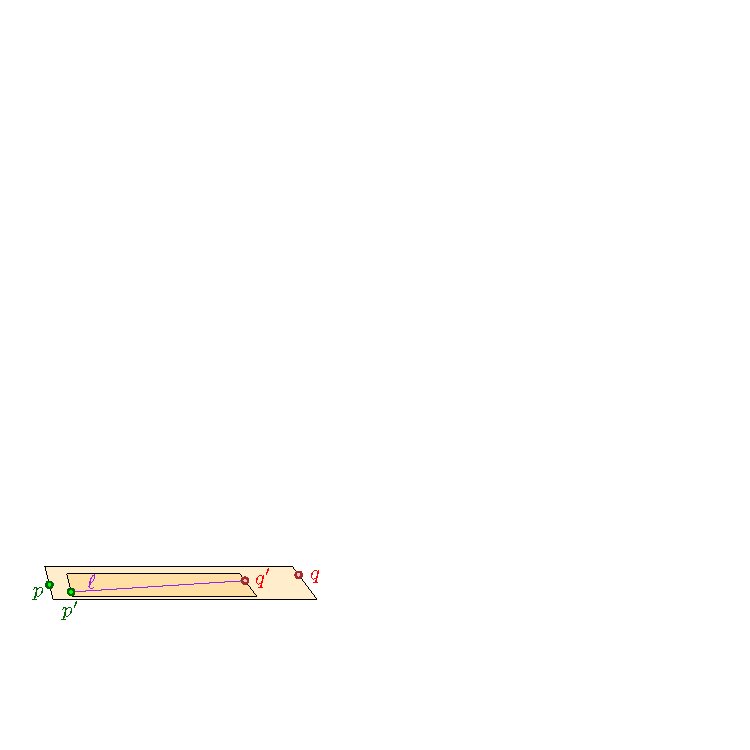
\includegraphics[width=0.3\linewidth]{../figs/narrow_trap}%
    \hfill%
    \includegraphics[page=2,width=0.3\linewidth]{../figs/narrow_trap}%
    \hfill%
    \includegraphics[page=3,width=0.3\linewidth]{../figs/narrow_trap}%
    \hfill\phantom{}%

    \phantom{}\hfill%
    (i)\qquad\qquad\qquad \hfill%
    (ii) \hfill%
    \qquad \qquad \qquad(iii) \hfill\phantom{}%

    \caption{Illustration of the settings in the proof of
       \lemref{good:jump:traps}. Left: A $\epsA$-narrow trapezoid with
       $\pa$ and $\pb$ on its legs. Center: $\pa$ and $\pb$ are
       $\epsA$-semi separated and $\epsA$-angularly separated. Right:
       The triangle of all the points of the trapezoids whose
       nearest point on $\pa \pb$ is $\pb$. }
    \figlab{narrow:trap}
\end{figure}


    Let $\ell = \dY{\pa'}{\pb'}$. Assume for concreteness that
    $\dY{\pa}{\pa'} \leq \diamX{\PX} \leq \epsA \dsY{\PX}{\PY} \leq
    \epsA \ell\leq \epsA \diamC$, where $\diamC=\diamX{\Trap}$. Let
    $\pb''$ be the closest point on $\pa\pb$ to $\pb'$.

    We first consider the case that $\pb'' \in \interiorX{\pa\pb}$.
    We have that
    \begin{equation*}
        \dY{\pa}{\pb''}
        =%
        \dY{\pa}{\pb'} \cos \angle \pb' \pa \pb
        \geq
        \bigl(\dY{\pa'}{\pb'} - \dY{\pa}{\pa'} \bigr)
        \cos \angle \pb' \pa \pb
        \geq
        (1-\epsA) \ell \cdot (1-\epsA^2/2)
        \geq
        (1-2\epsA) \ell,
    \end{equation*}
    since $\cos \epsA \geq 1-\epsA^2 /2$, for $\epsA <1/2$.  Similar
    arguments imply that $\dY{\pa}{\pb''} \leq (1+\epsA) \ell$. As
    such, we have
    \begin{equation*}
        \dY{\pb'}{\pb''} \leq ( 1+\epsA)\ell \sin \angle\pa'\pa \pb'
        \leq
        2 \epsA \ell.
    \end{equation*}
    Thus, we have that
    \begin{equation*}
        \dY{\pb}{\pb'}
        \leq
        \dY{\pb}{\pb''}  + \dY{\pb''}{\pb'}
        \leq%
        \dY{\pa}{\pb} -    \dY{\pa}{\pb''} + 2\epsA \ell
        \leq%
        \dY{\pa}{\pb} - (1-2\epsA)\ell + 2\epsA \ell
        \leq
        \dY{\pa}{\pb} - \ell.
    \end{equation*}

    and finally,
    \begin{align*}
      &(1+\eps)\dY{\pa}{\pa'} + \dY{\pa'}{\pb'} + (1+\eps)
        \dY{\pb'}{\pb}
        \leq%
        (1+\eps)\epsA \ell
        + \ell + (1+\eps)\bigl(
        \dY{\pa}{\pb} - \ell\bigr)
      \\&%
      \qquad=%
      (1+\eps)\dY{\pa}{\pb}
      +
      (1+\eps)\epsA \ell
      + \ell - (1+\eps)\ell
      \leq%
      (1+\eps)\dY{\pa}{\pb},
    \end{align*}
    for $\epsA \leq \eps/2$. Which establishes the claim in this case.

    The case $\pb''=\pa$ is impossible because of the angular
    separation property, and so, the only remaining possibility is
    that $\pb'' = \pb$. This however implies that $\pb'$ must be in
    the triangle of all the points of the trapezoid whose nearest
    point on $\pa \pb$ is $\pb$. The diameter of this triangle is
    bounded by the length of the leg of the trapezoid, which is
    bounded by $\epsA \, \diamC$. Namely, we have
    $\dY{\pb}{\pb'} \leq \epsA \diamC$. Similarly, we have
    \begin{math}
        (1 - 2\epsA) \diamC%
        \leq%
        \dY{\pa}{\pb} \leq%
        (1+2\epsA)\diamC.
    \end{math}
    Since $\dY{\pa}{\pa'}, \dY{\pb}{\pb'} \leq \epsA \diamC$, it
    follows that
    \begin{equation*}
        (1-4\epsA) \diamC%
        \leq%
        \ell%
        \leq%
        (1+4\epsA)\diamC.
    \end{equation*}
    As such, for $\epsA \leq \eps/8$ and $\eps \leq 1$, we have
    \begin{equation*}
        (1+\eps)\dY{\pa}{\pa'} + \ell + (1+\eps)
        \dY{\pb'}{\pb}
        \leq%
        4 \epsA \diamC + (1+4\epsA)\diamC
        =%
        (1+8\epsA)\diamC
        \leq
        (1+\eps) \dY{\pa}{\pb}.
    \end{equation*}
